% This is LLNCS.DOC the documentation file of
% the LaTeX2e class from Springer-Verlag
% for Lecture Notes in Computer Science, version 2.4
\documentclass{llncs}
\usepackage{llncsdoc}
\usepackage{url}
\usepackage[pdftex]{graphicx}     
\usepackage{float}
\usepackage{tablefootnote}
\usepackage{hyperref}



	%%%%%%%%%%%%%%%%%%%%%%%55
	%% Added to enable numbering for subsubsections, otherwise they would look like paragraphs which is ugly
	%%%%%%%%%%%%%%%%%%%%%%%55
	
	\makeatletter
	\renewcommand\subsubsection{\@startsection{subsubsection}{3}{\z@}%
		{-18\p@ \@plus -4\p@ \@minus -4\p@}%
		{0.5em \@plus 0.22em \@minus 0.1em}%
		{\normalfont\normalsize\bfseries\boldmath}}
	\makeatother
	\setcounter{secnumdepth}{3}

%
\begin{document}


	{
	%
	\title{title\\ \small Whitepaper}
	
	\author{Benjamin Leiding\inst{1} \and Will Vorobev\inst{1} \and Peter Zverkov\inst{1} \and Lena Cherry\inst{1}}
	
	\institute{ 
		Chorus Technology
	}
	
	%\institute{University of G\"ottingen, Institute of Computer Science, G\"ottingen, Germany\\ benjamin.leiding@cs.uni-goettingen.de
	%\and
	%Tallinn University of Technology, Department of Informatics, Tallinn, Estonia\\
	%alex.norta.phd@ieee.org}
	
	\maketitle

	%% ----------------------------------------------------------------
	%% ----------------------------------------------------------------

	\begin{abstract}

		% A good abstract:
		%1.) What is the paper about?
		%2.) What is the SoA?
		%3.) What is the detected gap?
		%4.) What are the main questions to be answered pertaining to the gap?
		%5.) Why is the solution good/better than other solutions?

		
		I am an abstract - pet me.

		
	\end{abstract}
	
	
	\keywords{keywords}

	%% ----------------------------------------------------------------
	%% ----------------------------------------------------------------
	
	\section{Introduction}
		\label{s:introduction}

	
		\textbf{Work-In-Progress}

		%https://www.heise.de/newsticker/meldung/Dubai-will-smarte-Kfz-Kennzeichen-testen-4016538.html


%%%%%%%%%%%%%%%%%%%%%%%%%%%%%%%%%%%%%%%%%%%%%%%%%%%%%%%%%%%%%%%%%%%%%%

%		RQ: How to ?
%		RQ-1: What ?
%		RQ-2: What ?
%		RQ-3: What are the system-engagement processes for the stakeholders?


%%%%%%%%%%%%%%%%%%%%%%%%%%%%%%%%%%%%%%%%%%%%%%%%%%%%%%%%%%%%%%%%%%%%%%

	


			The remainder of this paper is structured as follows: Section~\ref{s:section-2} introduces supplementary literature and related work. Section~\ref{s:section-3} then outlines the vision of Chorus Technology as well as different use-cases. Afterwards, Section~\ref{s:section-4} analyses the requirements of the our system and outlines the resulting system architecture that we derive from the requirements. Afterwards, Section~\ref{s:section-5} expands on the system-engagement processes for the stakeholders, followed by Section~\ref{s:section-6} that introduces the Chorus prototype as well as feasibility evaluation. Section~\ref{s:section-7} provides an discussion and an analysis of related projects. Finally, Section~\ref{s:section-8} concludes this work and provides an outlook on future work.


	%% ----------------------------------------------------------------
	%% ----------------------------------------------------------------

	\section{Technical Background and Related Works}	
		\label{s:section-2}
		
		The following section provides background information and describes related works regarding previous ideas and concepts that focus on a blockchain-based VANET platforms. First, Section~\ref{ss:blockchain-intro} introduces the general concepts of blockchain technology, terms and frameworks. Afterwards, Section~\ref{ss:autonomous-vehicles} and Section~\ref{ss:vanets} focus on the fundamentals of autonomous vehicles as well as vehicular ad-hoc networks. Finally, Section~\ref{ss:related-work} focuses on related work.	
					
		%% ----------------------------------------------------------------
		%% ----------------------------------------------------------------	
		
		\subsection{Blockchain Technology}
			\label{ss:blockchain-intro}
			
			\textbf{Work-In-Progress}				
			
			maybe already cite unchained and whisperkey paper?			
		
%			A blockchain consists of a chronologically ordered chain of blocks, where every block consists of a certain number of validated transactions. Each block links to its predecessor by a hash reference, so that changing the content of one block also changes all succeeding blocks and hence breaks the chain. All blocks are stored on and verified by all participating nodes. The blockchain concept is interesting for a M2M trading platform since it removes the need for trusted third party and instead enables trust-less transaction enactment and transactions that were agreed up on cannot be changed any more (tamper-proof).
%			
%			In recent years, the blockchain concept majored and spread in popularity. Besides the initial Bitcoin blockchain, several other architectures emerged, e.g., Ethereum \cite{wood2014ethereum}, Qtum \cite{qtumWhitepaper}, or Tezos \cite{tezosWhitepaper}. Those alternative blockchain platforms further provide Turing-complete programming languages on the protocol-layer level in order to enable smart contract capabilities. Smart contracts are, ``orchestration- and choreography protocols that facilitate, verify and enact with computing means a negotiated agreement between consenting parties" \cite{qtumWhitepaper}. Parties participating in the contract enactment establish binding agreements and deploy applications using such smart contracts in order to provide blockchain-based applications. Moreover, a variety of applications and use-cases for blockchains have been proposed, e.g., as a platform for IoT applications \cite{huckle2016internet}\cite{leiding2016self}, in the finance sector \cite{nguyen2016blockchain}\cite{tetherWhitepaper}, for reputation systems \cite{SemadaWhitepaper}, as part of security and authentication protocols \cite{AuthcoinLeiding2016MCIS}\cite{mccorry2015authenticated}\cite{ouaddah2017towards} or privacy solutions \cite{dorri2017blockchain}. 


		%% ----------------------------------------------------------------
		%% ----------------------------------------------------------------	
		
		\subsection{Autonomous Vehicles}
			\label{ss:autonomous-vehicles}

			\textbf{Work-In-Progress}
			
			%add the 5 autonomy levels as well as some definitions here

		%% ----------------------------------------------------------------
		%% ----------------------------------------------------------------	
		
		\subsection{Vehicular Ad-Hoc Networks - VANETs}
			\label{ss:vanets}

			\textbf{Work-In-Progress}
			
			%get stuff from the research projects as well as the ubicomp paper here
			
		%% ----------------------------------------------------------------
		%% ----------------------------------------------------------------	
		
		\subsection{Related Work}
			\label{ss:related-work}

			\textbf{Work-In-Progress}

			
%			Several other academic as well as non-academic projects experimented with ideas and prototypes of blockchain-based trading platforms that enable the M2M economy. In \cite{leiding2016self}, the authors describe a blockchain solution for a variety of services within vehicular ad-hoc networks (VANETs), e.g., traffic management, toll payment systems, traffic regulation enforcement and more. In 2018, the automotive company got a patent for a very similar idea of traffic marshaling via a blockchain system \cite{macneille2018vehicle}. Chorus technologies \cite{chorusWhitepaper} envisioned a whole library for all types of services and transaction around the ecosystem of autonomous vehicles within VANETs. The authors of \cite{davWhitepaper} propose a solution that allows vehicles to discover, communicate and transact with one another using cryptocurrencies. 
%			\cite{oakenTeslaTollbooth} present a prototype of a blockchain-based toll road system. In 2013, Mike Hearn gave a short talk\footnote{\url{https://www.youtube.com/watch?v=MVyv4t0OKe4}} at the Turing Festival in Edinburgh describing several of these ideas. 
%			
%			Besides the automotive sector, the authors of \cite{sikorski2017blockchain} describe and implement a M2M electricity market for chemical industry where industrial plants are trading electricity with each other via a blockchain platform.
%			
%			The alternative blockchain solution IOTA is offering an IoT market place \cite{iotaMarketplace} for IoT devices where sensor data can be bought and sold using blockchain technology.
%			
%		
		%% ----------------------------------------------------------------
		%% ----------------------------------------------------------------	
	

	%% ----------------------------------------------------------------
	%% ----------------------------------------------------------------

	\section{Longterm Vision}
		\label{s:section-3}
		
		Intro

		%foam and localization somewheere here	

		%% ----------------------------------------------------------------
		%% ----------------------------------------------------------------	
		
		\subsection{Use Cases}
			\label{ss:use-cases}

			\textbf{Work-In-Progress}
			
			\subsection{Human to Human}

			\subsection{Human to Vehicle}
		
			\subsection{Vehicle to Vehicle}
			
			\subsection{Vehicle to Infrastructure}					
		
		%% ----------------------------------------------------------------
		%% ----------------------------------------------------------------	


	%% ----------------------------------------------------------------
	%% ----------------------------------------------------------------
	
	
	\section{System Design and Architecture}
		\label{s:section-4}	

		Intro
		
		%% ----------------------------------------------------------------
		%% ----------------------------------------------------------------	
		
		\subsection{Functional Goals, Quality Goals, Stakeholders and Requirements}
			\label{ss:requirement-engineering}
			
			\textbf{Work-In-Progress}
			
			we leave out emotional goals here

			\begin{figure}[H]
				\centering
				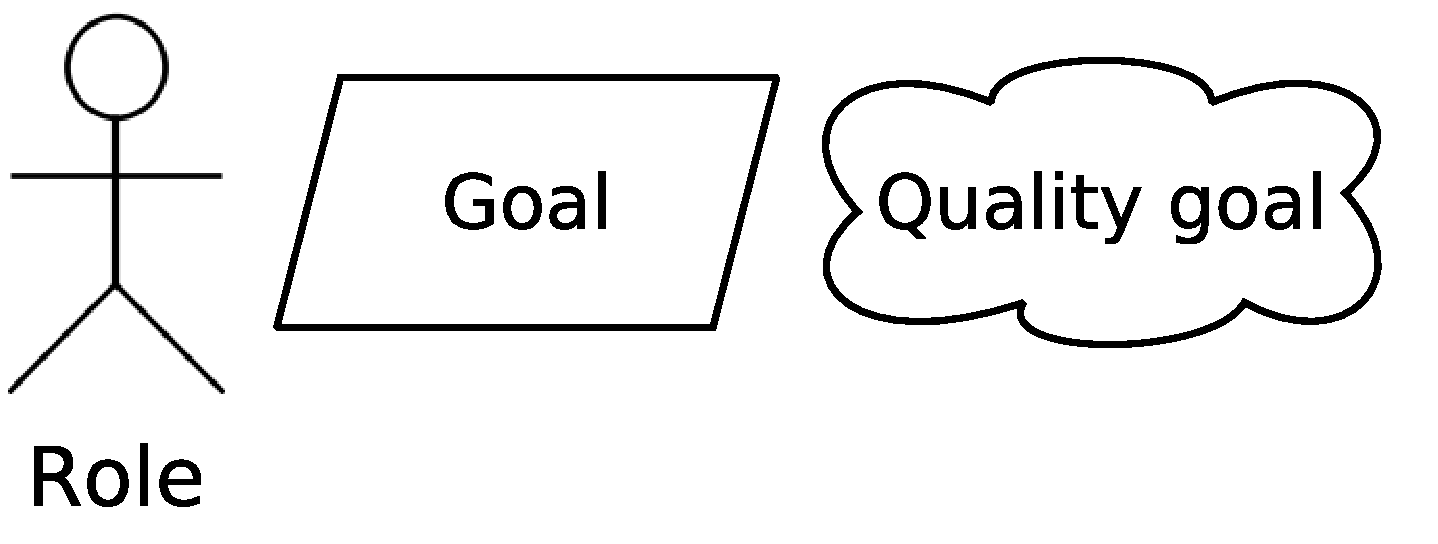
\includegraphics[scale=0.2]{Figures/20180426_AOM-notation.pdf}
				\caption{Selection of AOM notation elements.}	
				\label{fig:aom-notaion-elements}
			\end{figure}	
			
			%% ----------------------------------------------------------------
			%% ----------------------------------------------------------------	
					
			\subsubsection{Top-Level AOM Goal Model}
				\label{sss:top-level-goal-model}
			
			%% ----------------------------------------------------------------
			%% ----------------------------------------------------------------	
					
			\subsubsection{Refined AOM Goal Model}				
				\label{sss:refined-goal-model}			
	
			%% ----------------------------------------------------------------
			%% ----------------------------------------------------------------				

		%% ----------------------------------------------------------------
		%% ----------------------------------------------------------------	
		
		\subsection{High-Level Architecture}
			\label{ss:high-level-architecture}

		%% ----------------------------------------------------------------
		%% ----------------------------------------------------------------	
		
		\subsection{Component Diagrams}
			\label{ss:component-diagrams}

			\textbf{Work-In-Progress}

			\begin{figure}[H]
				\centering
				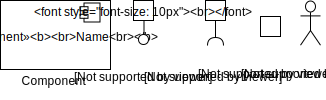
\includegraphics[scale=0.15]{Figures/UML-notation-elements.png}
				\caption{UML-component diagram notation elements.}	
				\label{fig:uml-component-diagram-overview}
			\end{figure}


		%% ----------------------------------------------------------------
		%% ----------------------------------------------------------------	

		\subsection{Smart Contract Lifecycle Management}

			\textbf{Work-In-Progress}
			
			%			The lifecycle of a micro lending contract is divided into the following stages: a) preparatory, b) negotiation, c) contract execution d) rollback and e) a contract expiry stage. During the preparatory stage, information about the involved entities, such as names and addresses are incorporated into the contract. In addition, the conditions of the requested loans are formally defined by specifying, e.g, the size of the loan, chosen currency, runtime and interest rates. The conditions of the requested loan mainly depend on information available to the lender, such as financial data gathered during previous interactions and transactions, personal data and information from social media. In case the borrower and the lender agree on the negotiated conditions, both parties sign the contract and express their approval - if no agreement is reached, a contract rollback is triggered. After signing the agreement, the contract execution phase is triggered and the lender transfers the loan to the borrower as illustrated in Figure \ref{fig:running-case-illustration}. Afterwards, the lender can use the loan to expand, or start a business. 
			%
			%			The micro lending contract terminates, or expires either after the defined loan timespan, or when the contract is prematurely terminated. The borrower pays back the loan either in separate rates, or as a whole, depending on the defined conditions. In addition, the lender also receives a fee, or an interest rate from the borrower for providing the loan. In case the borrower fulfills all his/her duties, the lender might provide a larger loan in the future based on the positive credit history of the borrower. Everex does not operate on the basis of P2P loans and instead invests its own aggregated capital to provide globally accessible credit services. Nevertheless, it is up to each Cryptocash owner to lend his/her own tokens to other users.	

		%% ----------------------------------------------------------------
		%% ----------------------------------------------------------------	
		
		\subsection{Library / API}
			\label{ss:library-api}				

			\textbf{Work-In-Progress}
			
		%% ----------------------------------------------------------------
		%% ----------------------------------------------------------------	

	%% ----------------------------------------------------------------
	%% ----------------------------------------------------------------
	
	\section{System Engagement Processes}
		\label{s:section-5}	
	
		Intro
		
		%describe processes here similar to evx paper

		%% ----------------------------------------------------------------
		%% ----------------------------------------------------------------	

		\subsection{Sequence Diagrams | or BPMN representation of Processes}

			\textbf{Work-In-Progress}

		%% ----------------------------------------------------------------
		%% ----------------------------------------------------------------	
		
		\subsection{Auction Algorithm}
			\label{ss:auchtion-algorithm}				

			\textbf{Work-In-Progress}

		%% ----------------------------------------------------------------
		%% ----------------------------------------------------------------	

		\subsection{Token Economics and Value Proposition}

			\textbf{Work-In-Progress}
					
		%% ----------------------------------------------------------------
		%% ----------------------------------------------------------------	

	%% ----------------------------------------------------------------
	%% ----------------------------------------------------------------

	\section{Prototype and Feasibility Study}
		\label{s:section-6}	
			
		Intro
		
		%% ----------------------------------------------------------------
		%% ----------------------------------------------------------------	
		
		\subsection{Prototype Scope}
			\label{ss:protoype-scope}				

			\textbf{Work-In-Progress}
			
					
		%% ----------------------------------------------------------------
		%% ----------------------------------------------------------------	
		
		\subsection{Evaluation}
			\label{ss:evaluation}				

			\textbf{Work-In-Progress}
			
					
		%% ----------------------------------------------------------------
		%% ----------------------------------------------------------------			

	%% ----------------------------------------------------------------
	%% ----------------------------------------------------------------

	\section{Discussion}
		\label{s:section-7}	
		
		Intro

		%% ----------------------------------------------------------------
		%% ----------------------------------------------------------------	
		
		\subsection{Critical Analysis}
			\label{ss:critical-analysis}
							
			\textbf{Work-In-Progress}		
		
		%% ----------------------------------------------------------------
		%% ----------------------------------------------------------------			
		
		\subsection{Related Work}
			\label{ss:competitor-analysis}
			
			%Competitor analysis (will)				

			\textbf{Work-In-Progress}
		
		%% ----------------------------------------------------------------
		%% ----------------------------------------------------------------					
	
	%% ----------------------------------------------------------------
	%% ----------------------------------------------------------------

	\section{Conclusion and Future Work}
		\label{s:section-8}	

		We conclude ...
		
		\textbf{Work-In-Progress}		
				
	%% ----------------------------------------------------------------
	%% ----------------------------------------------------------------


	\label{Bibliography}
	\bibliographystyle{splncs03}
	\bibliography{Bibliography}
	
	%% ----------------------------------------------------------------
	%% ----------------------------------------------------------------	



	%
\end{document}
